\graphicspath{{02-TOF/Figures/}}

\newcommand{\Tzero}{\ensuremath{T0}}
\newcommand{\Gauss}{\ensuremath{\text{G}}}
\newcommand{\DT}{\ensuremath{\Delta T}}
\newcommand{\us}{\ensuremath{\mu\text{s}}}

\section{Time-of-Flight Detectors}
\label{Sect:TOF}

% List of figures
% \begin{itemize}
% \item PMT charge correlation PMT0 vs PMT1 - maybe, if relevant
% \item \hilite{TW calibration of one channel}
% \item \hilite{Slab DT before TW correction and after - single pixel.}
% \item \hilite{Residual TW}
% \item T0 correction for 1 channel - electron peak fit
% \item \malert{(?)} Slab DT mean and sigma for all pixels after
%   calibration
%   \begin{itemize} \it
%   \item depends on whether we are comfortable with showing it
%   \end{itemize}
% \item \hilite{Overall slab DT}
% \item Space-point creation efficiency per pixel/slab
%   \begin{itemize}\it
%   \item this was tricky, the only inefficiency comes from time mismatch
%   \item it can point to a fact that some slabs/pixels have something
%     wrong with them
%   \item it was not measure of performance per se
%   \end{itemize}
% \item Particle detection efficiency
%   \begin{itemize} \it
%   \item don't know how to extract from the data, ideally pixel map for
%     each TOF
%   \end{itemize}

% \end{itemize}


% \malert{Issues:}
% \begin{itemize}
% \item should we use word ``counter'' or ``slab''?
% \end{itemize}

%%%%%%%%%%%%%%%%%%%%%%%%%%%%%%%%%%%%%%%%%%%%%%%%%%%%%%%%%%%%%%%%%%%%%%%%%%%%%%%%
\subsection{Introduction}
\label{SubSect:TOF_Intro}
% version 0.1 edited by Maurizio Bonesini 19/2/2018
% version 0.2 edited 23/10/2018

Three time-of-flight detectors (TOF0, TOF1, TOF2) were built and
installed at RAL in 2008 and 2009 to measure the position and the time
of crossing particles.  TOF0 and
TOF1~\cite{NOTE145}\cite{NOTE241}\cite{2010NIMPA.615...14B} were
placed upstream of the cooling channel, and TOF2~\cite{NOTE286} was
located downstream of the channel, mounted in front of the KLOE-Light pre-shower detector, as shown
in~figure~\ref{fig:BL}.
The time of flight between the first pair of TOF stations (figure~\ref{fig:TOF_peaks})
provided particle identification information and, assuming particles mass, can also be used to infer the momentum.
For most of the running, TOF1 served as an experimental trigger.
They operated smoothly during the 
running periods of the MICE experiment and were essential for all the
measurements that were performed~\cite{Rajaram:2015bra}\cite{2015ehep.confE.521B}.

\begin{figure}[!ht]
  \begin{center}
    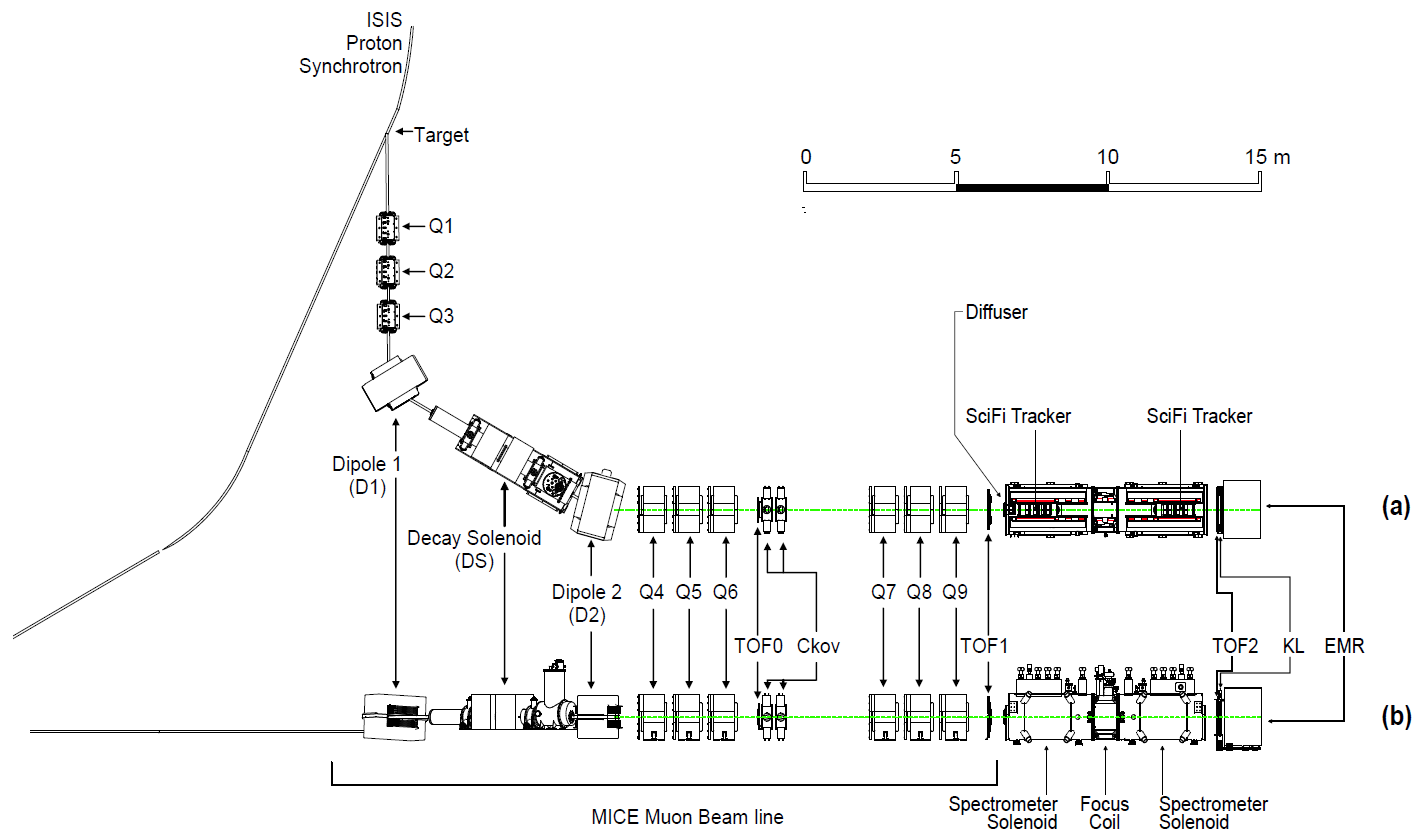
\includegraphics[width=0.8\columnwidth]{BL.png}
    \caption{MICE, showing the full beam line starting from the target position on the proton synchrotron) with the full set of quadrupoles and dipoles (Q1 to Q9, D1/2), the Decay Solenoid, and cooling channel elements with all the detectors. The liquid-hydrogen absorber vessel inside the Focus Coil is shown in figure~\ref{Fig:AbsorberVessel:Diag}}.
    \label{fig:BL}
  \end{center}
\end{figure}

The good performance of the TOF and KL detectors, over an extended period of time,
enabled the MICE experiment to fully characterise its muon beams during
the early stages of data-taking, by measuring their emittance~\cite{2013arXiv1306.1509T} and assessing their pion contamination~\cite{2016JInst..11P3001A}.

Each TOF station was made of two planes of 1'' scintillator bars oriented along X and Y directions, respectively.
The bars were made of BC-404 plastic scintillator. A simple fishtail light-guide was used to attach each end of each bar to R4998 Hamamatsu fast photomultiplier tubes,
enclosed in assemblies that included the voltage divider chain and a 1\,mm thick $\mu$-metal shield. To increase the count-rate stability, active
dividers were used. The TOF detector is illustrated in figure~\ref{fig:tof:schematic}.

%%%%Mu-metal is a nickel–iron soft ferromagnetic alloy with very high permeability, which is used for shielding sensitive electronic equipment against static or low-frequency magnetic fields.

\begin{figure}[!ht]
  \centering
  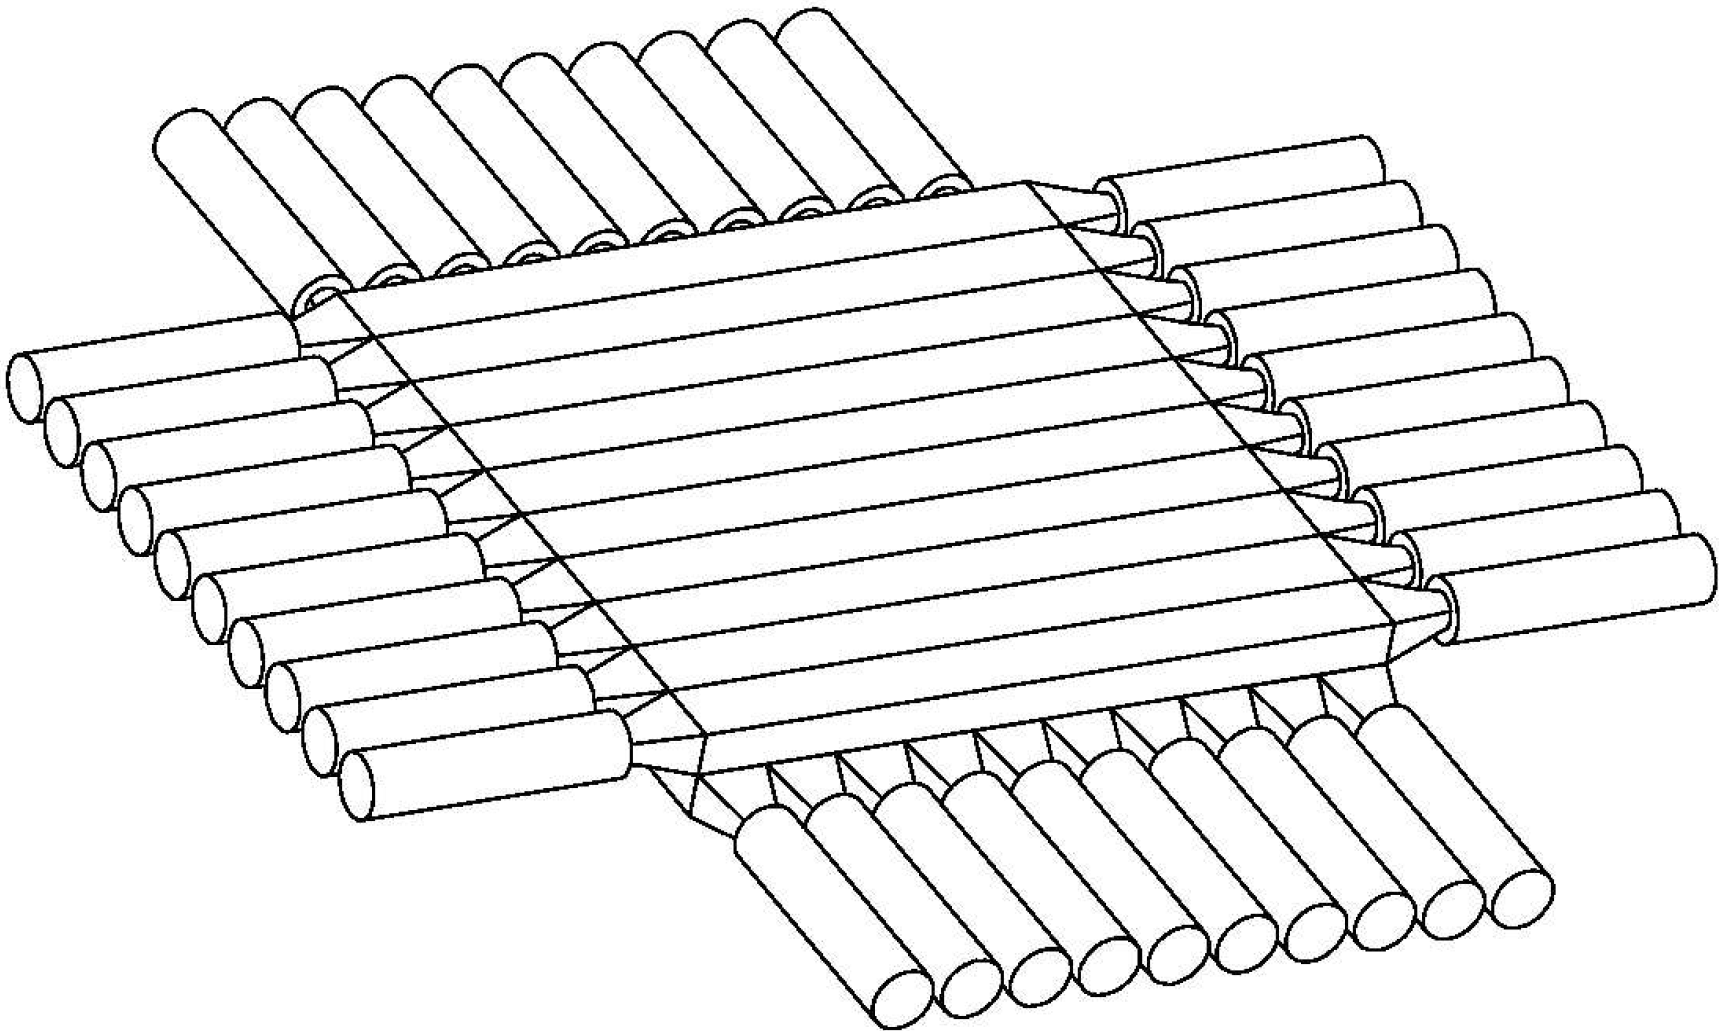
\includegraphics[width=8cm]{tof_diagram2}
  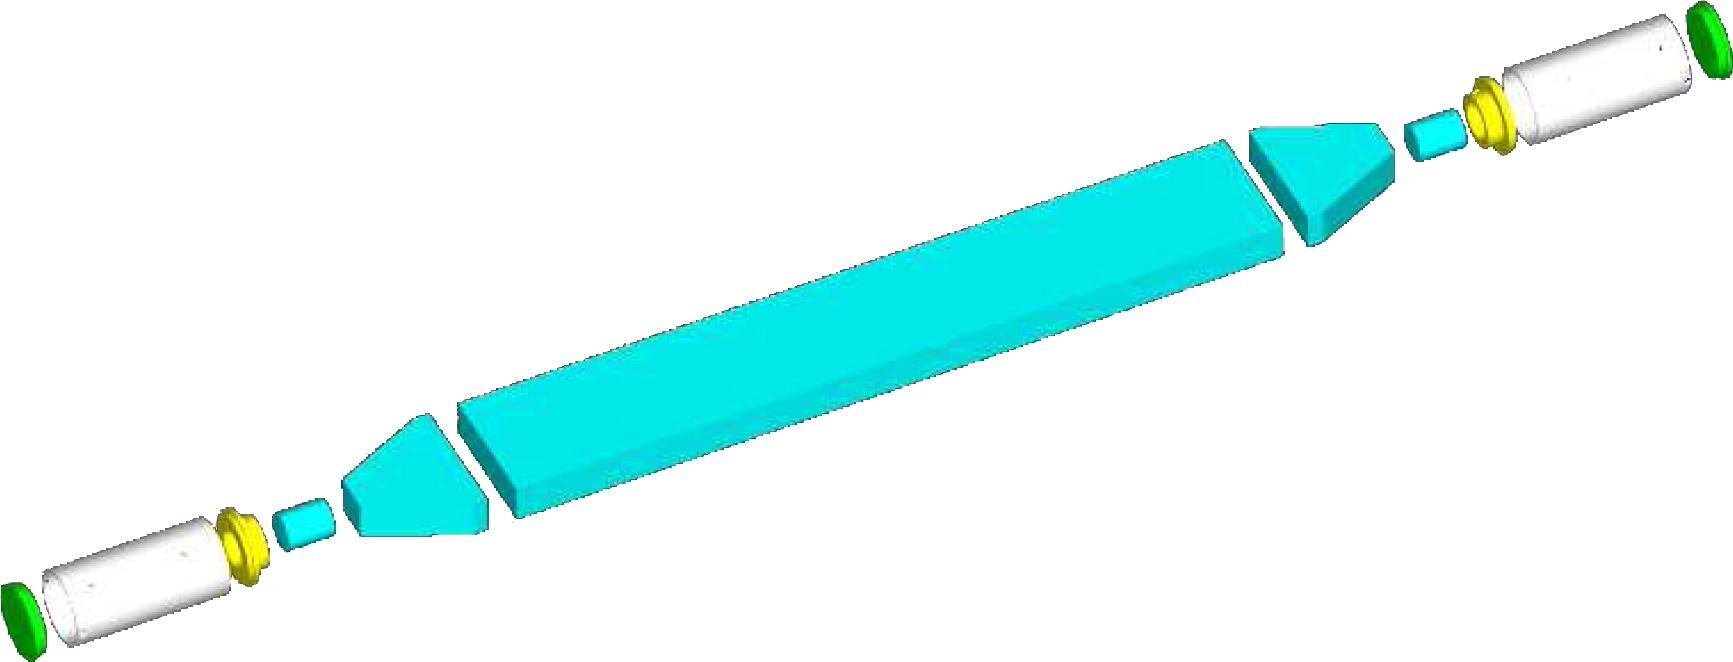
\includegraphics[height=3cm]{slab_design2}
  \caption{Design of the TOF detector structure showing the horizontal and vertical layers of slabs (left) and exploded view of each slab showing one scintillator with the light-guides and the PMTs (right) on each side~\cite{NOTE145}.}
  \label{fig:tof:schematic}
\end{figure}

The three stations TOF0, TOF1, and TOF2 had active areas of
40$\times$40\,cm$^2$, 42$\times$42\,cm$^2$, and 60$\times$60\,cm$^2$
respectively.  Each of the planes in TOF0 had 10, 4\,cm wide, scintillator slabs.
Stations TOF1 and TOF2 were composed by 7 and 10 scintillator slabs in each plane, respectively.
The PMTs were connected to a passive splitter.
One half of the signal was fed to the leading-edge CAMAC Lecroy 4115 discriminator followed by a CAEN
V1290 TDC for time measurement and the second half of the signal went to a CAEN V1724 FADC for pulse-height measurement.
%Pulse height measurement was essential for time-walk corrections.
Each electronic channel issued a local readout trigger if signals in both PMTs attached to a
slab crossed a specific threshold. All three stations were read out when the TOF1 station issued a local trigger.
This readout trigger was also used for the rest of the MICE detector systems.

% Pulse heights and times of the signals were recorded if
%\malert{Do we want to include this?:}
% As reported in
%reference~\cite{NOTE241}, RG213 cables\footnote{CERN type C-50-6-1,
%  with rated delay 4.08 ns/m} have a better temperature stability than
%conventional RG58 cables.

% \malert{Unnecessary: Their delay have been individually measured in laboratory, before installation in the experimental hall.  Time  calibration of individual counters has been done with impinging beam  particles by using the detector X/Y redundancy~\cite{NOTE251}. }

All stations were exposed to residual magnetic fields: TOF0 was placed in a relatively low residual field produced by the last quadrupole magnet of the beam line (which had mirror plates installed), while the other two TOF stations were exposed to the stray fields of the cooling channel solenoids. A shielding structure was adopted covering all PMTs at each side of the stations~\cite{2010NIMPA.615...14B}.

%All three stations were exposed to residual magnetic fields. TOF0 station was placed in a relatively low residual field ($\le 5\,\Gauss$) produced by the last quadrupole magnet of the beam line.  The PMTs in this station used 1-mm thick $\mu$-metal shielding \malert{(we don't seem to have any reference)}. The other two TOF stations (TOF1/TOF2) were exposed to the stray fields of the cooling channel solenoids that were only partially shielded by 10\,mm thick annular iron plates \malert{(need to have a reference, possibly described earlier in the  paper)}. The residual magnetic fields were up to 0.13~T (with a component along the PMTs axis up to 0.04~T). Box-shaped soft iron shielding was more effective than cylindrical one.

% too much about the shielding, removed.
%This idea, pioneered in the D0 experiment \malert{(citation needed, or remove altogether)}, has been
%tested in the case of MICE using different geometrical configurations
%of the iron shielding boxes and different iron materials (e.g. Fe360,
%ARMCO\footnote{ARMCO steel from AkSteel was a pure iron with a maximal
%  carbon content of $0.025\%$ and very high magnetic
%  saturation},~etc) \cite{2012NIMPA.693..130B}.
% Systematic studies were
% performed~\cite{2012NIMPA.693..130B} and
%A composite structure of the shielding was adopted. The first layer of
%the shielding consisted of 1~mm $\mu$-metal around the Hamamatsu
%H6533Mod assemblies. The second layer was an additional box-shaped
%ARMCO bulk with a borehole of 3.2~cm in diameter~\cite{NOTE455} for
%each PMT. A single-bar-like structure was used to shield all PMTs at
%each side of the station. The bars were 15~cm deep, and 5.7~cm or
%6.6~cm thick for TOF1 or TOF2, respectively.  \malert{(Original text
%  stated 6$\times$6~cm$^2$ anfd 5.6$\times$5.6~cm$^2$, 15~cm
%  long. This was with contradiction with the design drawings in MICE
%  note 455 (TOF1) and the drawing provided in this paper (TOF2))}
%figure~\ref{fig:TOF1} shows the design drawing of the shielding at the
%TOF2 station detailing individual parts. There was an extra shielding
%effect due to the fact that all bars of the TOF2 PMTs were
%magnetically linked together and also linked to both the KL shielding
%and the shielding plate \malert{(which shielding plate)} making a
%single magnetic loop.
%\begin{figure}
%  \begin{center}
%  \includegraphics[width=9cm,angle=-90]{./02-TOF/Figures/TOF2.eps} \\
%  \caption{Exploded view of the TOF2 detector magnetic shielding for
%    one row of PMTs. Visible are different pieces of ARMCO shielding
%    and the plastic holder and end-caps (left) for mounting the bases of
%    individual PMTs.}
%  \label{fig:TOF1}
%  \end{center}
%\end{figure}

% \malert{The following paragraph was summarising the performance. It
%   states overly optimistic performance.}
% \malert{reformulate ---} For what attains performances\malert{---},
% TOF0, TOF1, and TOF2 had timing resolutions around 50-60 ps
% respectively \malert{(currently observed $\sim$110~ps)}, over the 8
% years running period, consistent with design requirements, with the
% spatial resolution around 1~cm. \malert{We don't use any special
%   reconstruction method. Resolution kept at 4 cm or 6 cm for TOF0 or
%   TOF1 and TOF2 respectively. Do we say resolution = 1/2 of strip
%   width or $1/\sqrt{12}$?}  figure~\ref{fig:TOF3}~shows distributions of
% the time of flight between TOF0 and TOF1 where electrons, muons and
% pions fall into three well defined peaks.
% \begin{figure}
%   \begin{center}
%     \includegraphics[width=8cm]{./02-TOF/Figures/TOF.png}
%     \caption{Time of flight between TOF0 and TOF1 for a ``pion''
%       beam. From the left: the well separated electron, muon and pion
%       peaks.}
%     \label{fig:TOF3}
%   \end{center}
% \end{figure}

% \malert{What was currently the main purpose of TOFs? This determines
%   the requirements on the performance. Will need to tell that current
%   T-o-F measurement has sufficient resolution, which appears to be
%   $\sim$100-120~ps}

The purpose of the TOF system was to discriminate particle species
based on time-of-flight measurement. The main components in the
MICE beam were muons, pions, and positrons. The time resolution needed
to be sufficiently good to effectively discriminate between these
types. At 240\,MeV/$c$, the time-of-flight difference between a muon and
a pion was about 1.3\,ns between the TOF0 and the TOF1 stations. With 200\,ps
resolution, together with momentum information, we reached near 100\% discrimination efficiency~\cite{Bogomilov:2012sr}.


%%%%%%%%%%%%%%%%%%%%%%%%%%%%%%%%%%%%%%%%%%%%%%%%%%%%%%%%%%%%%%%%%%%%%%%%%%%%%%%%
%The following text describes the method used to calibrate the TOF system and its performance.

\subsubsection{Calibration Method}
% \begin{itemize}
% \item Describe the method. Based on MICE note 251.
% \item \malert{TOF NIMA paper says that measured time resolution of the
%     CAEN TDC was 22~ps/count, as opposed  to declared 25~ps!}
% \item  Some description of the calibration method was also described in the
%   paper.
% \item  \malert{There's a short description of the method also in Rayner's
%     Thesis, Section 3.2.1 and Appendix B (this was improved method to
%     extract more calibration constants for proper x,y measurements,
%     Rayner claims $\sim$1~cm resolution; our current resolution = slab
%     width / sqrt(12) $\sim 1.2 - 1.7$ ).}
% \end{itemize}

Determination of time stamp of a particle through a TOF station was
influenced by several factors at the hardware level.

When a particle crossed the plastic scintillator, there was a short delay in light
production, with a characteristic decay time of 1.8\,ns.
After generation, scintillation light propagates to the ends of each
scintillator slab where it was detected by photomultiplier tubes. The
light-travel time depends on the distance of the particle crossing
from the PMT. The lengths of slabs in TOF0, TOF1, and TOF2 were 40\,cm,
40\,cm, and 60\,cm, respectively. This translates to about 3.0\,ns, 3.1\,ns,
and 4.4\,ns of light travel time, respectively, as the effective light
propagation speed in the scintillator was found to be approximately
13.5\,cm/ns.  More delay was introduced by the transit time of each PMT
and of the cable that led the signal to the readout electronics. These
times were unique for each individual PMT channel and needed to be
determined in dedicated measurements.

A simple linear discriminator measured the time of each signal coming from a PMT.
This introduced bias in the measured time dependent on the total charge of the signal, an effect referred to as time-walk.

Signal times of each channel were recorded in TDC boards. Readout of
the whole system was triggered by having a signal in TOF1. The
readout trigger signal was distributed to all TDC boards and was used as
a reference time. Which PMT channel's threshold crossing caused the
readout was dependent on where the particle crossed through the TOF1
station. As a consequence, the reference time had a bias dependent on
the position of the TOF1 crossing, an effect referred to here as trigger
delay. To compensate this, the final time measurement in each station was determined as an average of the times of individual channels.
%This way, different distances from the point of crossing to each side of the scintillator slabs does not matter anymore, because the average of the times of the 2 PMTs does not depend on it.

Corrections which needed to be made to the measured times were then the
time-walk correction, the PMT channel specific delay time and
a correction for the reference trigger time delay~\cite{NOTE251}.

%%%%%%%%%%%%%%%%%%%%%%%%%%%%%%%%%%%%%%%%%%%%%%%%%%%%%%%%%%%%%%%%%%%%%%%%%%%%%%%%
\subsubsection{Reconstruction}

A particle crossing a TOF station must have crossed at least 2 orthogonal slabs
in the station's 2 planes.  The time and approximate position of
a particle crossing a TOF station was reconstructed from the PMT signals
in the two slabs. Each slab with at least one recorded signal in each
of the 2 PMTs was considered as being crossed by a
particle. Times of these recorded signals were corrected for
time-walk, readout trigger signal delay, and the channel specific
delay. Time of crossing of the slab was then taken as the average of
the 2 corrected PMT times.

The 2 slabs hit by a particle defined a pixel of area given by the
width of the slabs. Sometimes, there were more slabs in each plane
with signals. Matching of 2 slabs being crossed by a particle was done
based on their measured signal time. They were matched if the times
were within a 4\,ns window. The time of the particle crossing was
determined as the average of times of the 2 matched slabs.

% In order to be able to correct for the trigger signal delay, the pixel
% through which the particle crossed TOF1 needed to be determined. All
% possible combinations of 2 slabs from 2 different planes were
% tested. The times of the recorded PMT signals were corrected under the
% hypothesis that correct slabs were matched.

%%%%%%%%%%%%%%%%%%%%%%%%%%%%%%%%%%%%%%%%%%%%%%%%%%%%%%%%%%%%%%%%%%%%%%%%%%%%%%%%
\subsection{Performance}
\label{SubSect:TOF_Performance}

% \malert{Several figures are already in the TOF NIMA paper.}

% Figures to show here:
% \begin{itemize}
% \item Slab DT - selected slabs/counters + overall TOFs
% \item ToF10 - + detail of electron peak
%   \begin{itemize} \it
%   \item will need to argue why the peak was broader than stated
%     resolution
%   \item the effect of electron's flight path due to focusing fields is
%     non-negligible - use estimates from Rayner's thesis
%   \end{itemize}
% \item Space-point reconstruction efficiency
%   \begin{itemize}
%   \item shows that slab hits are within the required cut
%     \begin{itemize}
%     \item events with 2 slab hits only
%     \end{itemize}
%   \item inefficiency from:
%     \begin{itemize}
%     \item only single slab hit by different particles in the given
%       spill/bunch
%     \item this may be due to inefficiency of hit creation when
%       particle crosses by the edge of the slab -- see Rayner's
%       thesis/presentations
%     \item two particles share one slab - earlier particle's hit only
%       considered - but this was not considered in these plots (only 2
%       slab hits recorded)
%     \end{itemize}
%   \end{itemize}
% \item Stability of electron peak - run by run position of electron peak!
% \item particle detection efficiency - how to show?
% \item Resolution
%   \begin{itemize}
%   \item Slab DT for all TOFs, show similar performance, although
%     they have different construction.
%   \end{itemize}
% \item \malert{(?)}Efficiency
% \end{itemize}

The resolution of the time-of-flight measurement was given by time resolution
of each station.
The time associated to each TOF was determined from the average of the times when the two slabs (horizontal and vertical) were crossed by a particle.
The resolution of the average was a half of the spread of their difference. Therefore, looking at slab \DT{} allowed the time-of-flight
resolution to be determined.

%Due to the errors in calibrations, especially in the underpopulated
%peripheral pixels, the slab \DT{} distributions have slight offsets
%from 0. Also, the spread of the distributions varies from pixel to
%pixel. The offsets and the spreads of the slab \DT{} distributions for
%individual pixels are shown in
%Figures~\ref{fig:SlabDToffsetByPixel}~and~\ref{fig:SlabDTresByPixel},
%respectively.

Overall performance can be inferred from the combined slab \DT{}
distributions. The plots in figure~\ref{fig:SlabDtAll} show that they
all centre approximately at 0\,ns and they exhibit very similar
resolutions, with TOF1 having the largest spread.
Figure~\ref{fig:TOF_peaks} shows an example of measurement of time of
flight between the first two stations, TOF0 and TOF1. Flight times of electrons,
muons, and pions are clearly separated, creating peaks from left to
right, respectively. The observed width of the electron peak of
approximately~0.10\,ns was about 30\%~larger than the calculated spread from a
naive addition of slab \DT{} of the individual TOF stations.
This difference was attributed to contributions to the resolution of
individual stations which cancel out in the slab \DT{} measurement,
and to variations in the travelled path length of the electrons between
stations TOF0 and TOF1.

\begin{figure}
  \begin{center}
  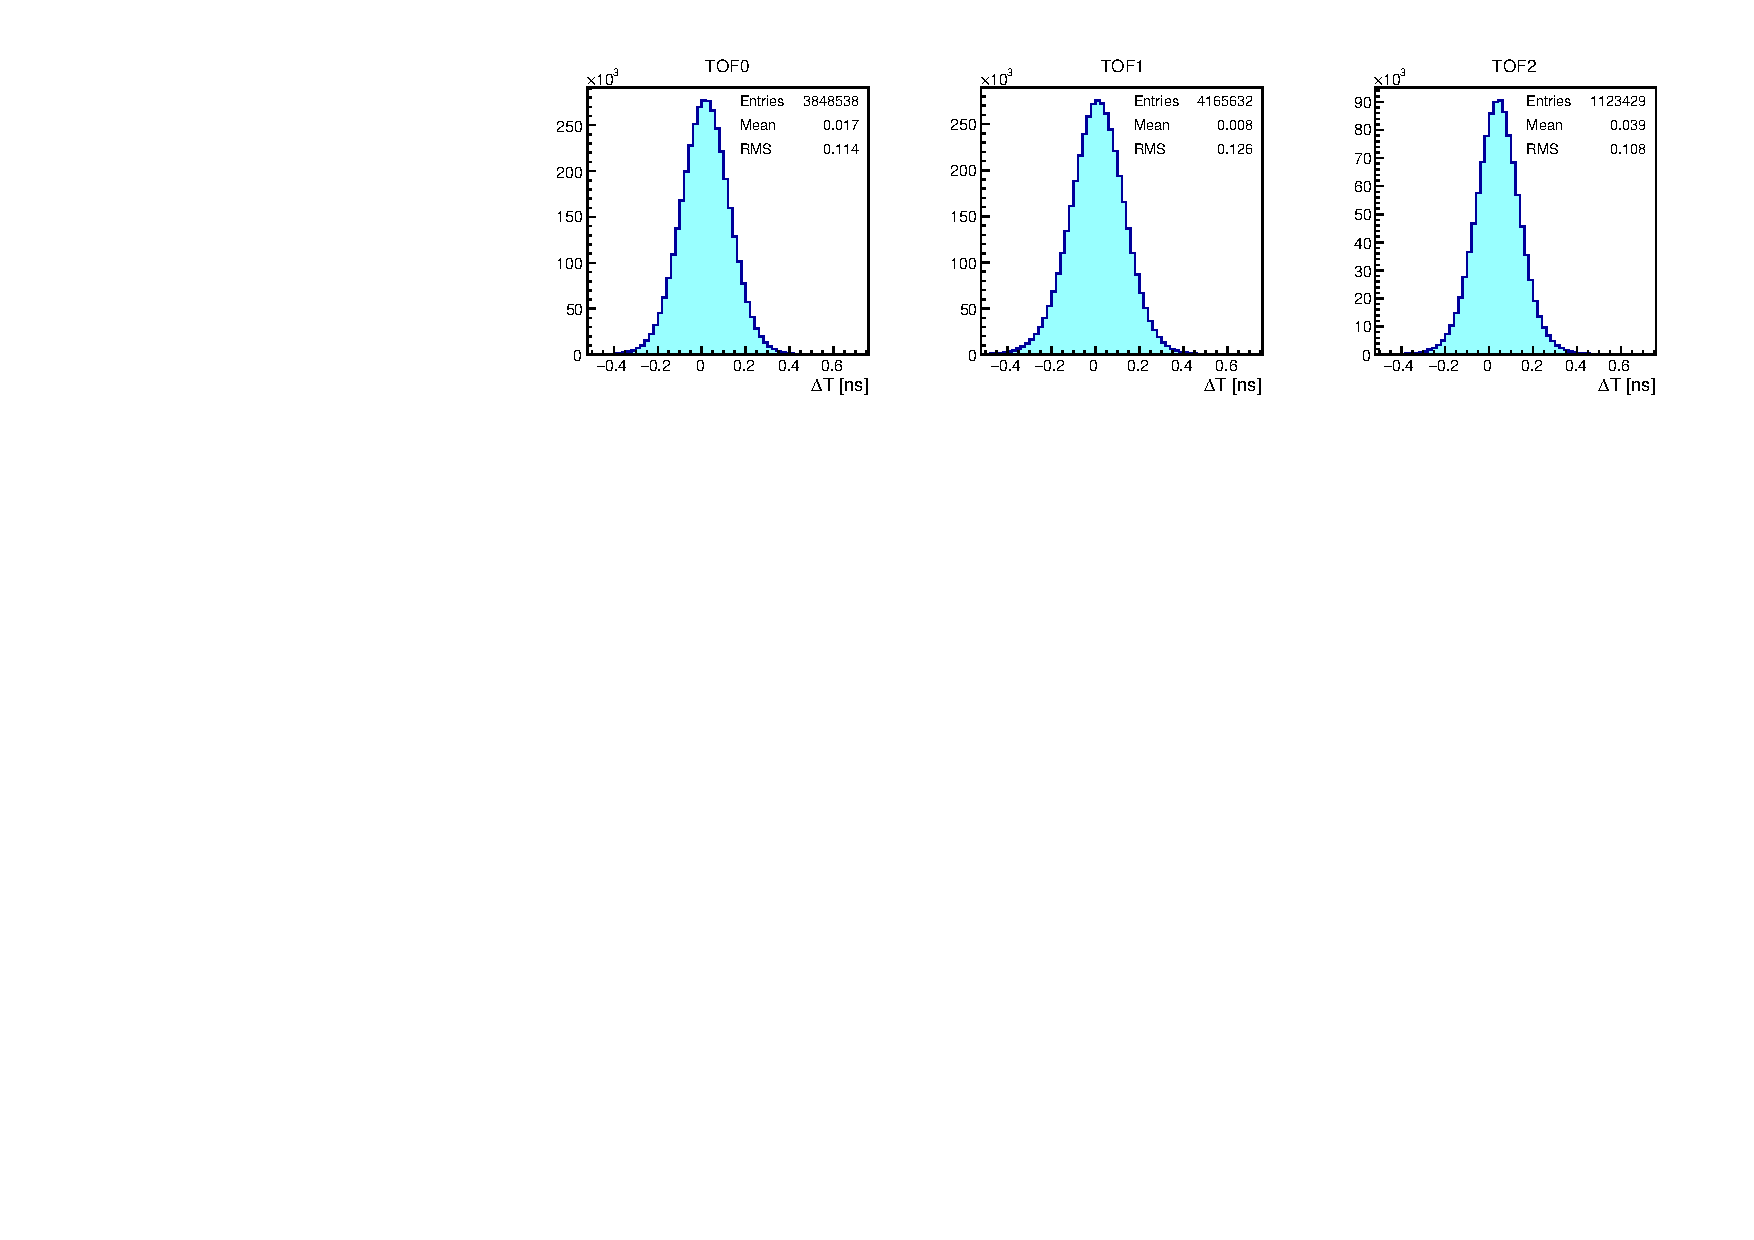
\includegraphics[width=0.9\columnwidth]{07_overall_slab_dt} \\
  \caption{Overall slab \DT{} distributions. Total width of the
    distribution was due to the resolution of individual pixels and due to
    the offsets in their \DT{} distributions.}
  \label{fig:SlabDtAll}
  \end{center}
\end{figure}

% Error of the time-of-flight measurement was a combination of intrinsic
% resolution of each TOF station and errors in the calibrations of
% individual \malert{scintillation counters}. The total error of t-o-f
% as measured by stations $i$ and $j$ was considered as:
% %
% \begin{equation}
%   \label{eq:tof:err}
%   \sigma_{\text{TOF}_{ij}} = \sqrt{ \sigma^2_{i} + \sigma^2_{j} +
%     \sigma^2_{\text{calib}} } .
% \end{equation}
% %
% Individual uncertainties $\sigma_i$ are assumed to be statistically
% uncorrelated. Error of the calibration method, $\sigma_\text{calib}$,
% consists of uncertainties correlated and uncorrelated between the
% stations.

% The reconstruction of a pixel by matching of 2 slabs from different
% planes of each station was dependent on the slab \DT{}. The 4~ns time
% window for the matching was chosen to cover the errors of the
% calibrations. Yet, there were times when there were signals in slabs
% in each plane of a station, but they were never matched. These events
% were mostly results of multiple particles passing through the station
% and causing signal in one plane only. They would never be matched in
% time as they arrived within the beam bunch time stretch of about
% 1~\us{}.
%Figure~\ref{fig:SpEffByPixel} shows fractions of events where
%there were signals in two perpendicular slabs and they were
%time-matched. One can see lower efficiency/fraction in the peripheral
%pixels which was associated with the larger fraction of multiple
%particle crossings with giving signal in one slab only.


%To be changed with a better one
\begin{figure}[!htb]
  \begin{center}
    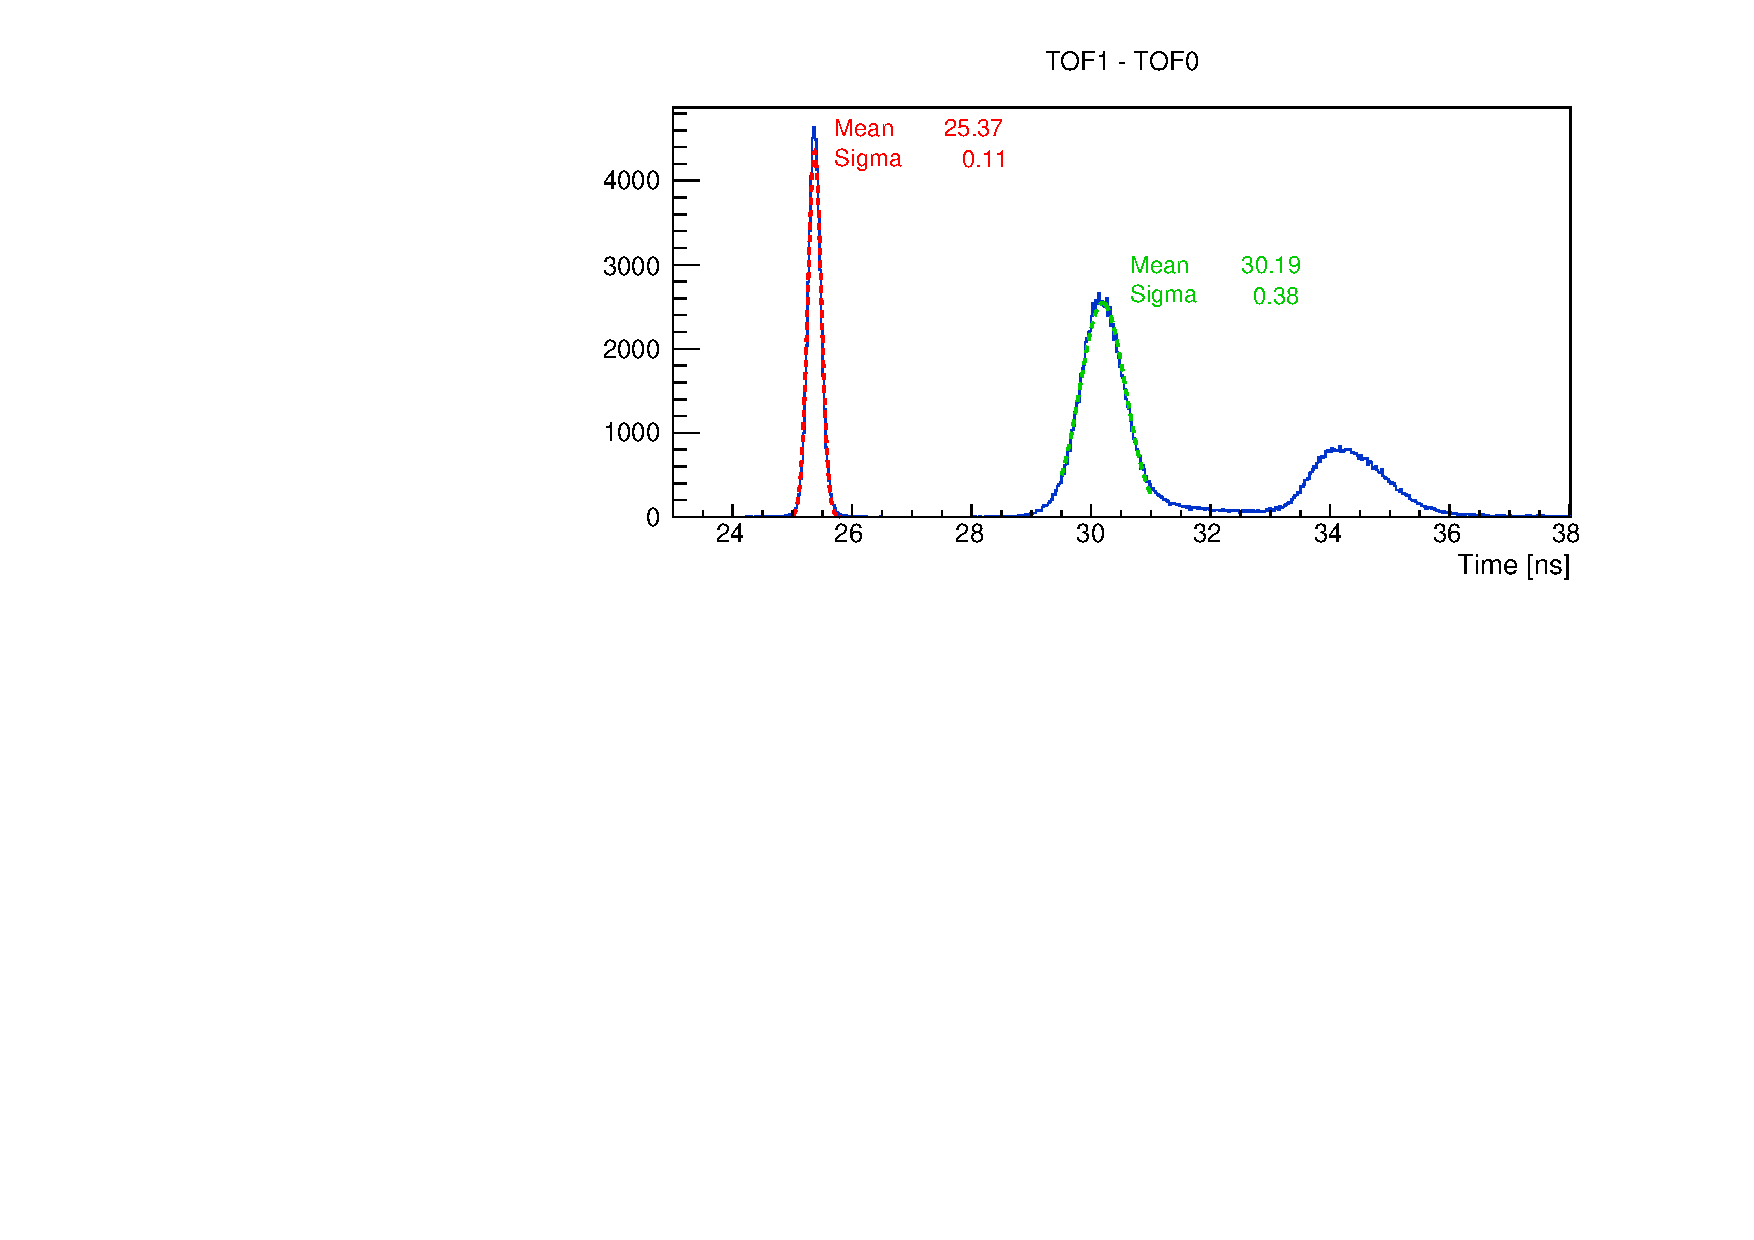
\includegraphics[width=0.6\columnwidth]{TOF_peaks.pdf}
    \caption{Time of flight between TOF0 and TOF1 for a ``pion'' beam
      after all corrections have been applied. From the left: the well
      separated electron, muon and pion peaks.}
    \label{fig:TOF_peaks}
  \end{center}
\end{figure}

%%%%%%%%%%%%%%%%%%%%%%%%%%%%%%%%%%%%%%%%%%%%%%%%%%%%%%%%%%%%%%%%%%%%%%%%%%%%%%%%

% \subsubsection{Low-level Characterisation}

% \malert{maybe leave this out, likely not necessary}

% \begin{itemize}
% \item PMT charge correlation PMT0 vs PMT1 - maybe, if relevant
% \item Residual TW - this should go to the calibration section
% \item Slab DT
% \end{itemize}

% \subsubsection{Time-of-Flight Resolution and Efficiency}

% \begin{itemize}
% \end{itemize}
